%   ------------------------------------------------------------------------
\FloatBarrier
\subsection{Geração da animação de pulo}
\label{s.gemini.animacaoPular}

Para a geração da animação de pulo, foi possível utilizar a versão final do sprite em side view (Figura \ref{fig:geminiProPabloPixelLabSide}). Como foi dito anteriormente, a análise irá desconsiderar o conteúdo sonoro do vídeo.

O resultado inicial\footnote{\url{https://drive.google.com/file/d/131HVD9P7_fZnAPsjHeYBHitE1ipKgKCG/view?usp=sharing}} gerado apresentou alta consistência com o sprite, conseguindo gerar uma animação parcialmente coerente com o estilo de pixel art. No início do vídeo, o personagem começa sem olho (Figura \ref{fig:GeminiProPularSemOlho}), porém o mesmo é gerado de forma precisa antes do movimento. Formaram-se distintos pulos no mesmo vídeo, onde os braços e as pernas ficavam de maneiras diferentes. Além disso, as mãos se deformam ao longo do vídeo, como pode ser visto na Figura \ref{fig:GeminiProPularMaoDeformacao}. Interação completa pode ser consultada na Figura
\ref{fig:geminiProPular1} no Apêndice \ref{ap.telasIA}.

\begin{figure}[htbp]
    \centering
    \begin{minipage}{0.45\textwidth}
        \centering
        \caption{\small Sprite sem o olho na animação de pulo gerado no Gemini Pro}
        \label{fig:GeminiProPularSemOlho}
        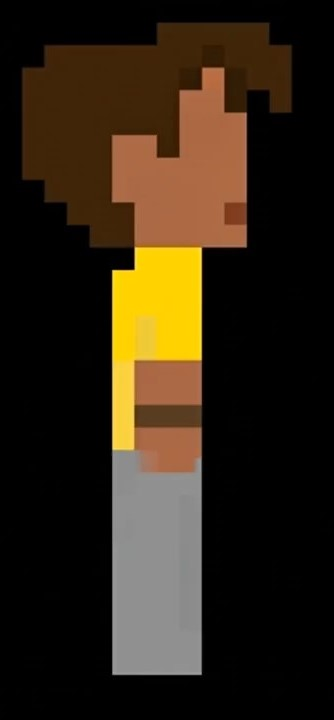
\includegraphics[width=0.5\linewidth]{figs/geminiPro/chat7/semOlho.jpg}
        \legend{\small Fonte: Elaborada pela autora, utilizando a ferramenta Gemini Pro.}
    \end{minipage}\hfill
    \begin{minipage}{0.45\textwidth}
        \centering
        \caption{\small Sprite com a mão deformada na animação de pulo gerado no Gemini Pro}
        \label{fig:GeminiProPularMaoDeformacao}
        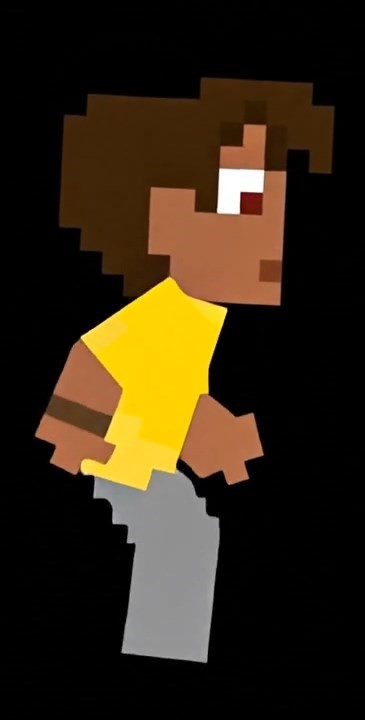
\includegraphics[width=0.5\linewidth]{figs/geminiPro/chat7/maoDeformada.jpg}
        \legend{\small Fonte: Elaborada pela autora, utilizando a ferramenta Gemini Pro.}
    \end{minipage}
\end{figure}


No teste posterior (Figura \ref{fig:geminiProPular2} no Apêndice \ref{ap.telasIA}), tentou-se incluir o deslocamento horizontal do pulo na animação através de um prompt que instruía a edição do vídeo já gerado sem anexo de uma nova imagem de referência. O resultado\footnote{\url{https://drive.google.com/file/d/1XS2euWjdv9dG-pvYUYqbuyQoUXlcfjfo/view?usp=sharing}} não se moveu para o lado, porém apresentou menos deformações na mão, manteve o movimento do pulo constante e preciso, sem movimentos extras das pernas e dos braços. Além disso, a coerência com a pixel art continuou e apenas a consistência do bracelete diminuiu, como mostra a Figura \ref{fig:geminiProPularMaoMelhor}. Dessa forma, sua qualidade foi considerada melhor do que a da animação anterior.

\begin{figure}[htbp]
    \centering
    \caption{\small Sprite da animação de pulo com o bracelete inconsistente gerada no Gemini Pro}
    \label{fig:geminiProPularMaoMelhor}
    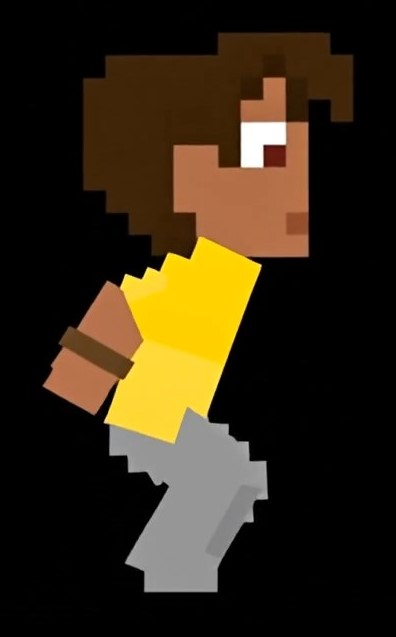
\includegraphics[width=0.3\linewidth]{figs/geminiPro/chat7/maoCerta.jpg}
    \legend{\small Fonte: Elaborada pela autora, utilizando a ferramenta Gemini Pro.}
\end{figure}


Depois foi notado que o deslocamento deve ser realizado pela movimentação física do objeto no Unity, onde o sprite fica mudando de acordo com o frame de forma que sempre esteja centralizado com o colisor. Assim, não é necessário que o personagem se mova de um ponto A para um ponto B no vídeo gerado, inclusive essa movimentação apenas torna mais complicado o processo de manter o sprite visível na mesma posição do objeto.

Apesar do conteúdo já ser satisfatório, mais experimentos foram realizados em busca de um resultado com menos falhas. Porém, todos os vídeos gerados\footnote{\url{https://drive.google.com/drive/folders/1nC_Mn9xHSIVC97XQD9yduLMBAohsexgx?usp=sharing}} apresentaram mais erros de consistência nas mãos e nos braceletes (Figura \ref{fig:geminiProPularInconsistente}). Além disso, formaram-se movimentos exagerados durante o pulo. Os testes podem ser verificados nas Figuras \ref{fig:geminiProPular3} a \ref{fig:geminiProPular5} no Apêndice \ref{ap.telasIA}.

\begin{figure}[htbp]
    \centering
    \caption{\small Sprite inconsistente da animação de pulo gerada no Gemini Pro}
    \label{fig:geminiProPularInconsistente}
    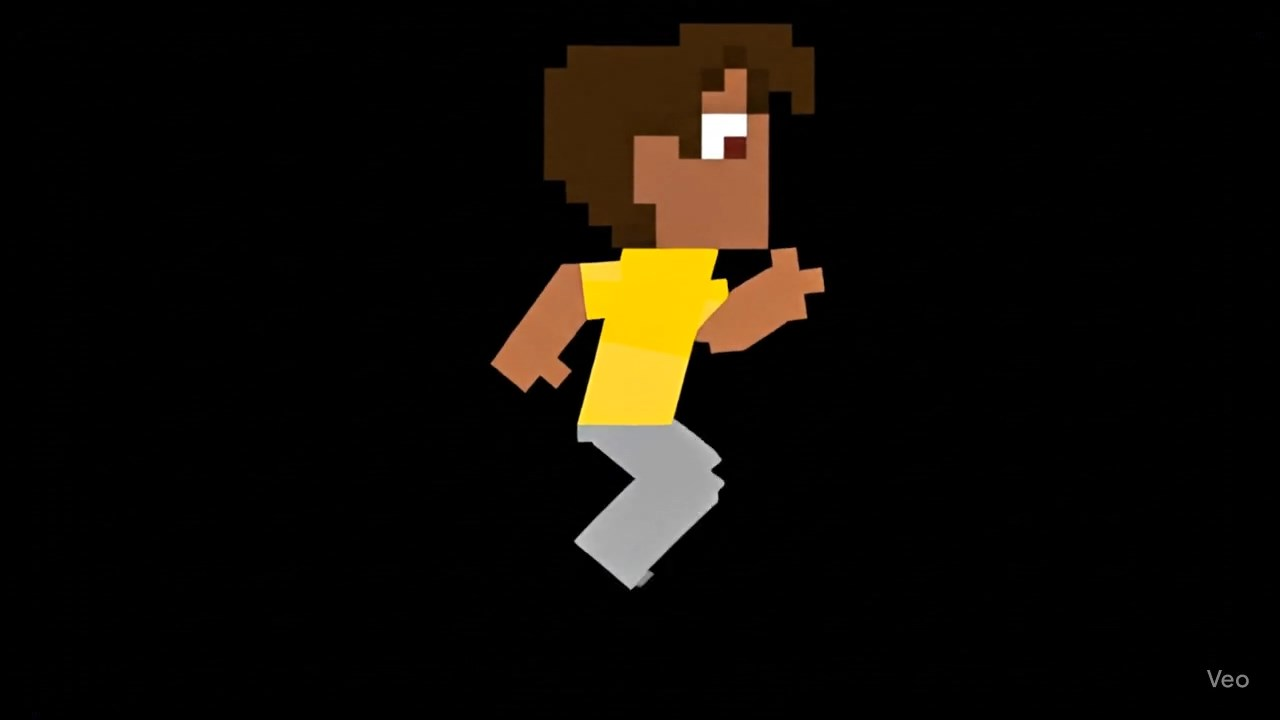
\includegraphics[width=0.6\linewidth]{figs/geminiPro/chat7/print17.jpg}
    \legend{\small Fonte: Elaborada pela autora, utilizando a ferramenta Gemini Pro.}
\end{figure}


Dessa forma, a Figura \ref{fig:geminiProPular2} no Apêndice \ref{ap.telasIA} foi considerada o melhor resultado. O sprite sheet do vídeo foi extraído através do ezgif (mencionado anteriormente), demonstrado na Figura \ref{fig:geminiProPularSpriteSheet}. Essa imagem foi cortada de forma a conter a animação de um único pulo, como pode ser vista na Figura \ref{fig:geminiProPularSpriteSheetCortado}. 

\begin{figure}[htbp]
    \centering
    \caption{\small Sprite sheet completo da animação de pulogerada no Gemini Pro}
    \label{fig:geminiProPularSpriteSheet}
    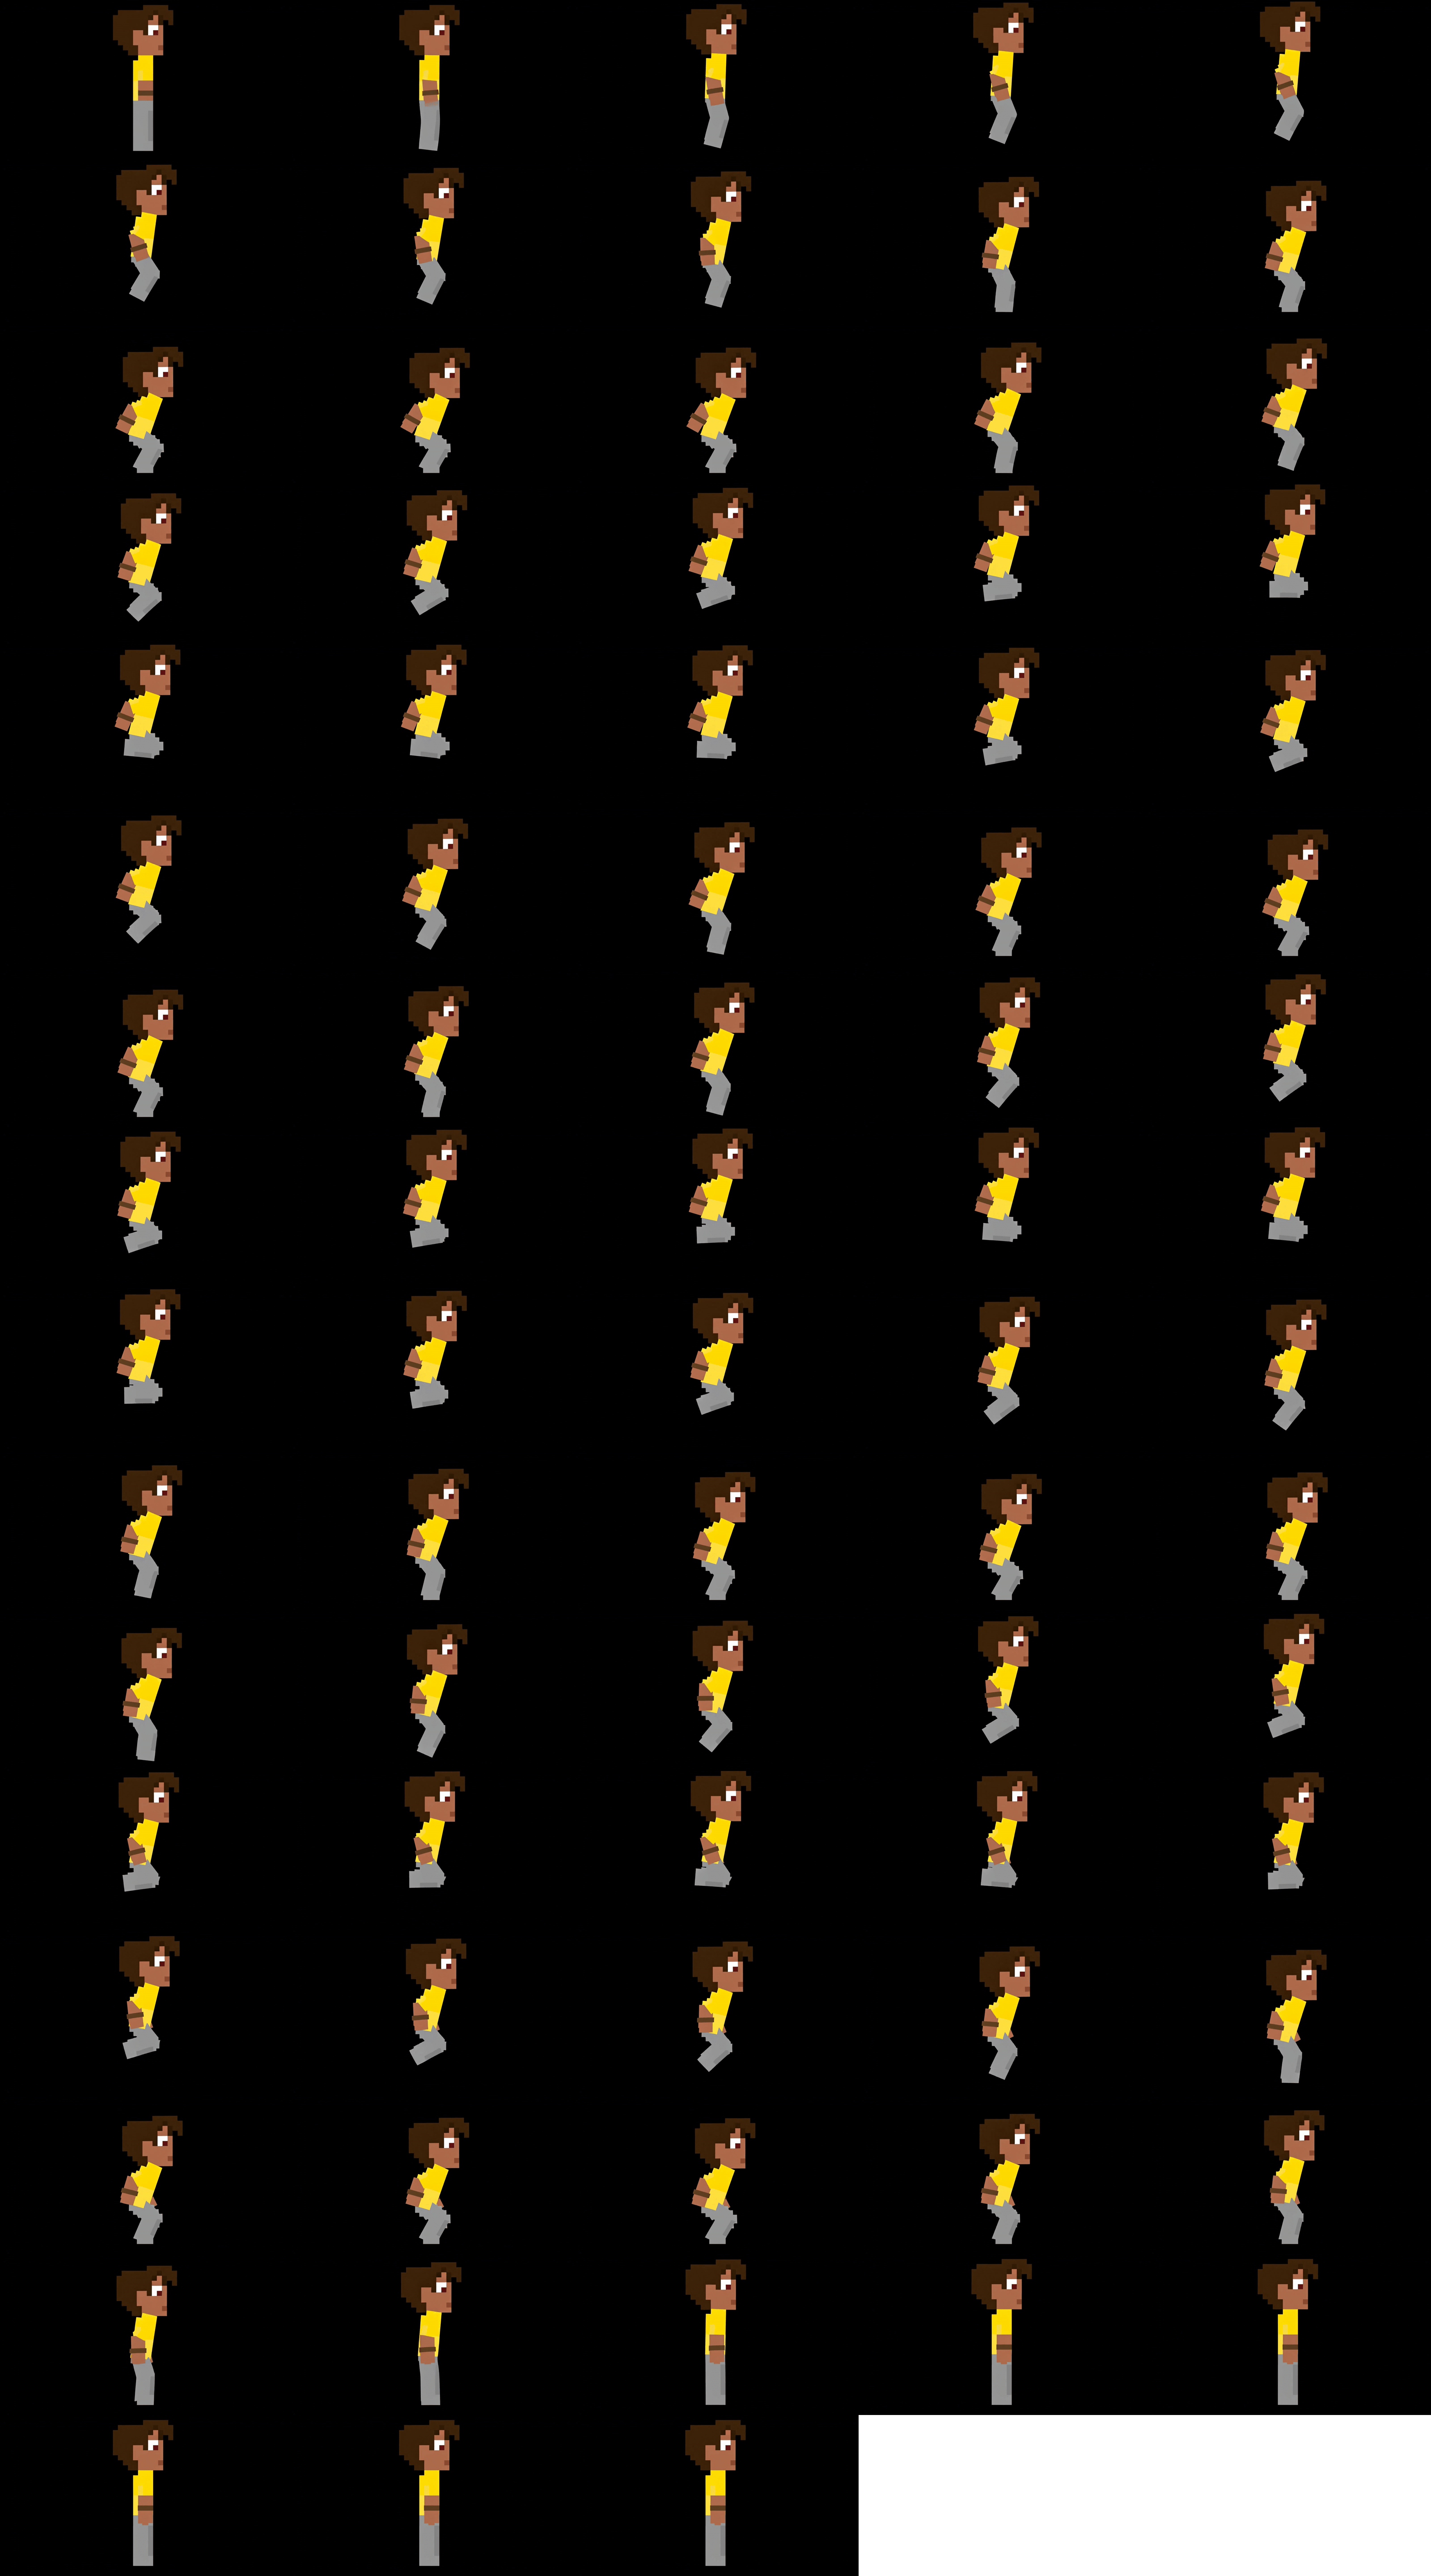
\includegraphics[width=0.6\linewidth]{figs/geminiPro/sprite sheet/jump.png}
    \legend{\small Fonte: Elaborada pela autora, utilizando a ferramenta ezgif.}
\end{figure}

\begin{figure}[htbp]
    \centering
    \caption{\small Sprite sheet cortado da animação de pulo gerada no Gemini Pro}
    \label{fig:geminiProPularSpriteSheetCortado}
    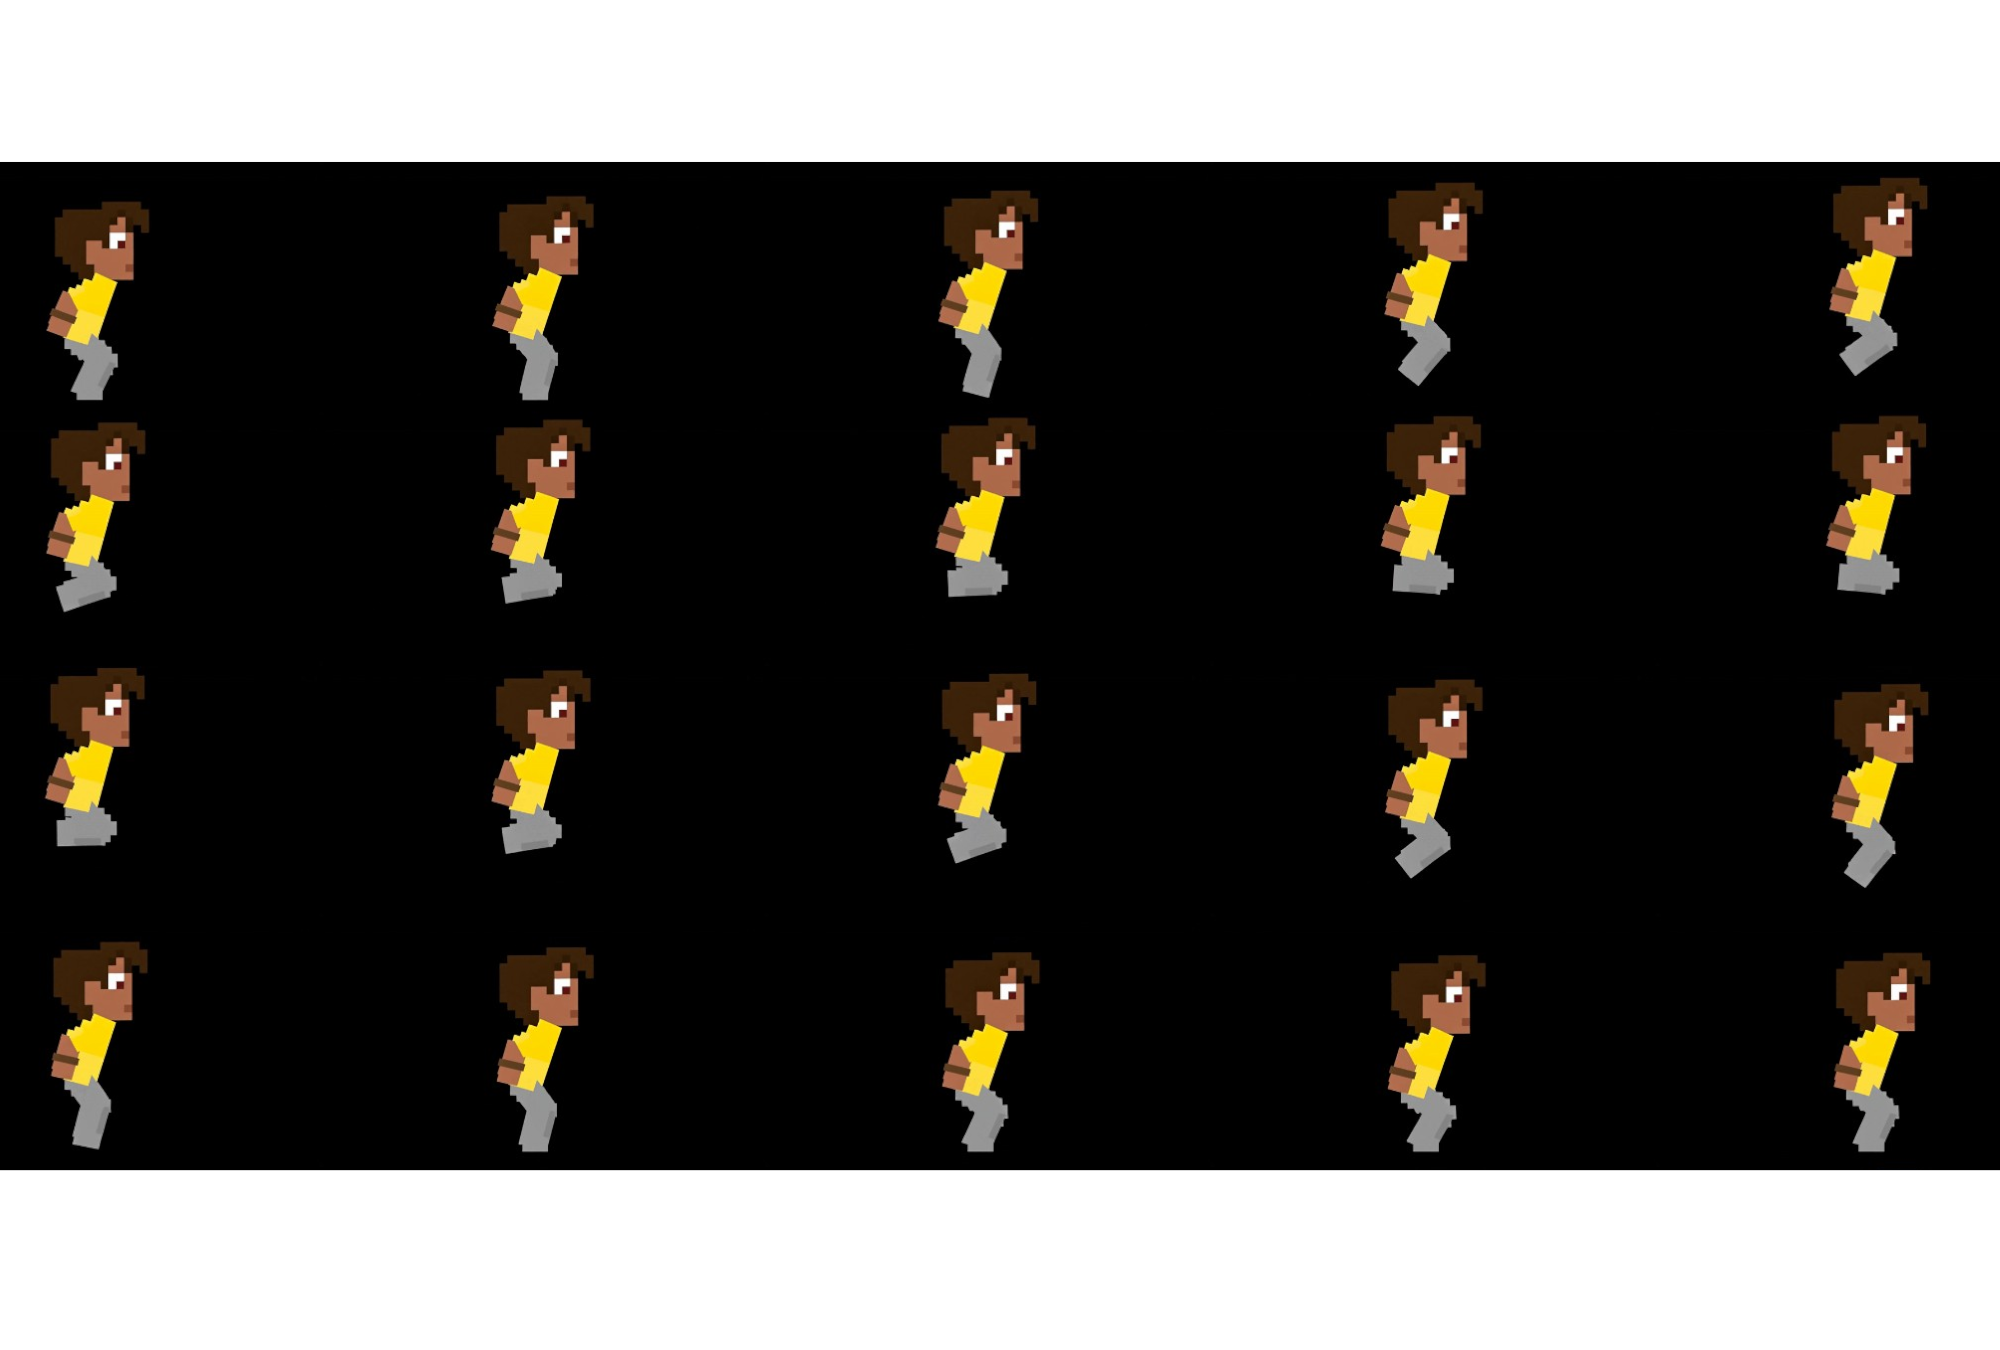
\includegraphics[width=0.8\linewidth]{figs/geminiPro/sprite sheet/jump_corte.png}
    \legend{\small Fonte: Elaborada pela autora, utilizando a ferramenta ezgif.}
\end{figure}

Após isso, o fundo da imagem é retirado com o auxílio da ferramenta removebg (mencionada anteriormente), resultando na Figura \ref{fig:geminiProPularSpriteSheetTransparente}.

\begin{figure}[htbp]
    \centering
    \caption{\small Sprite sheet com fundo transparente da animação de pulo gerada no Gemini Pro}
    \label{fig:geminiProPularSpriteSheetTransparente}
    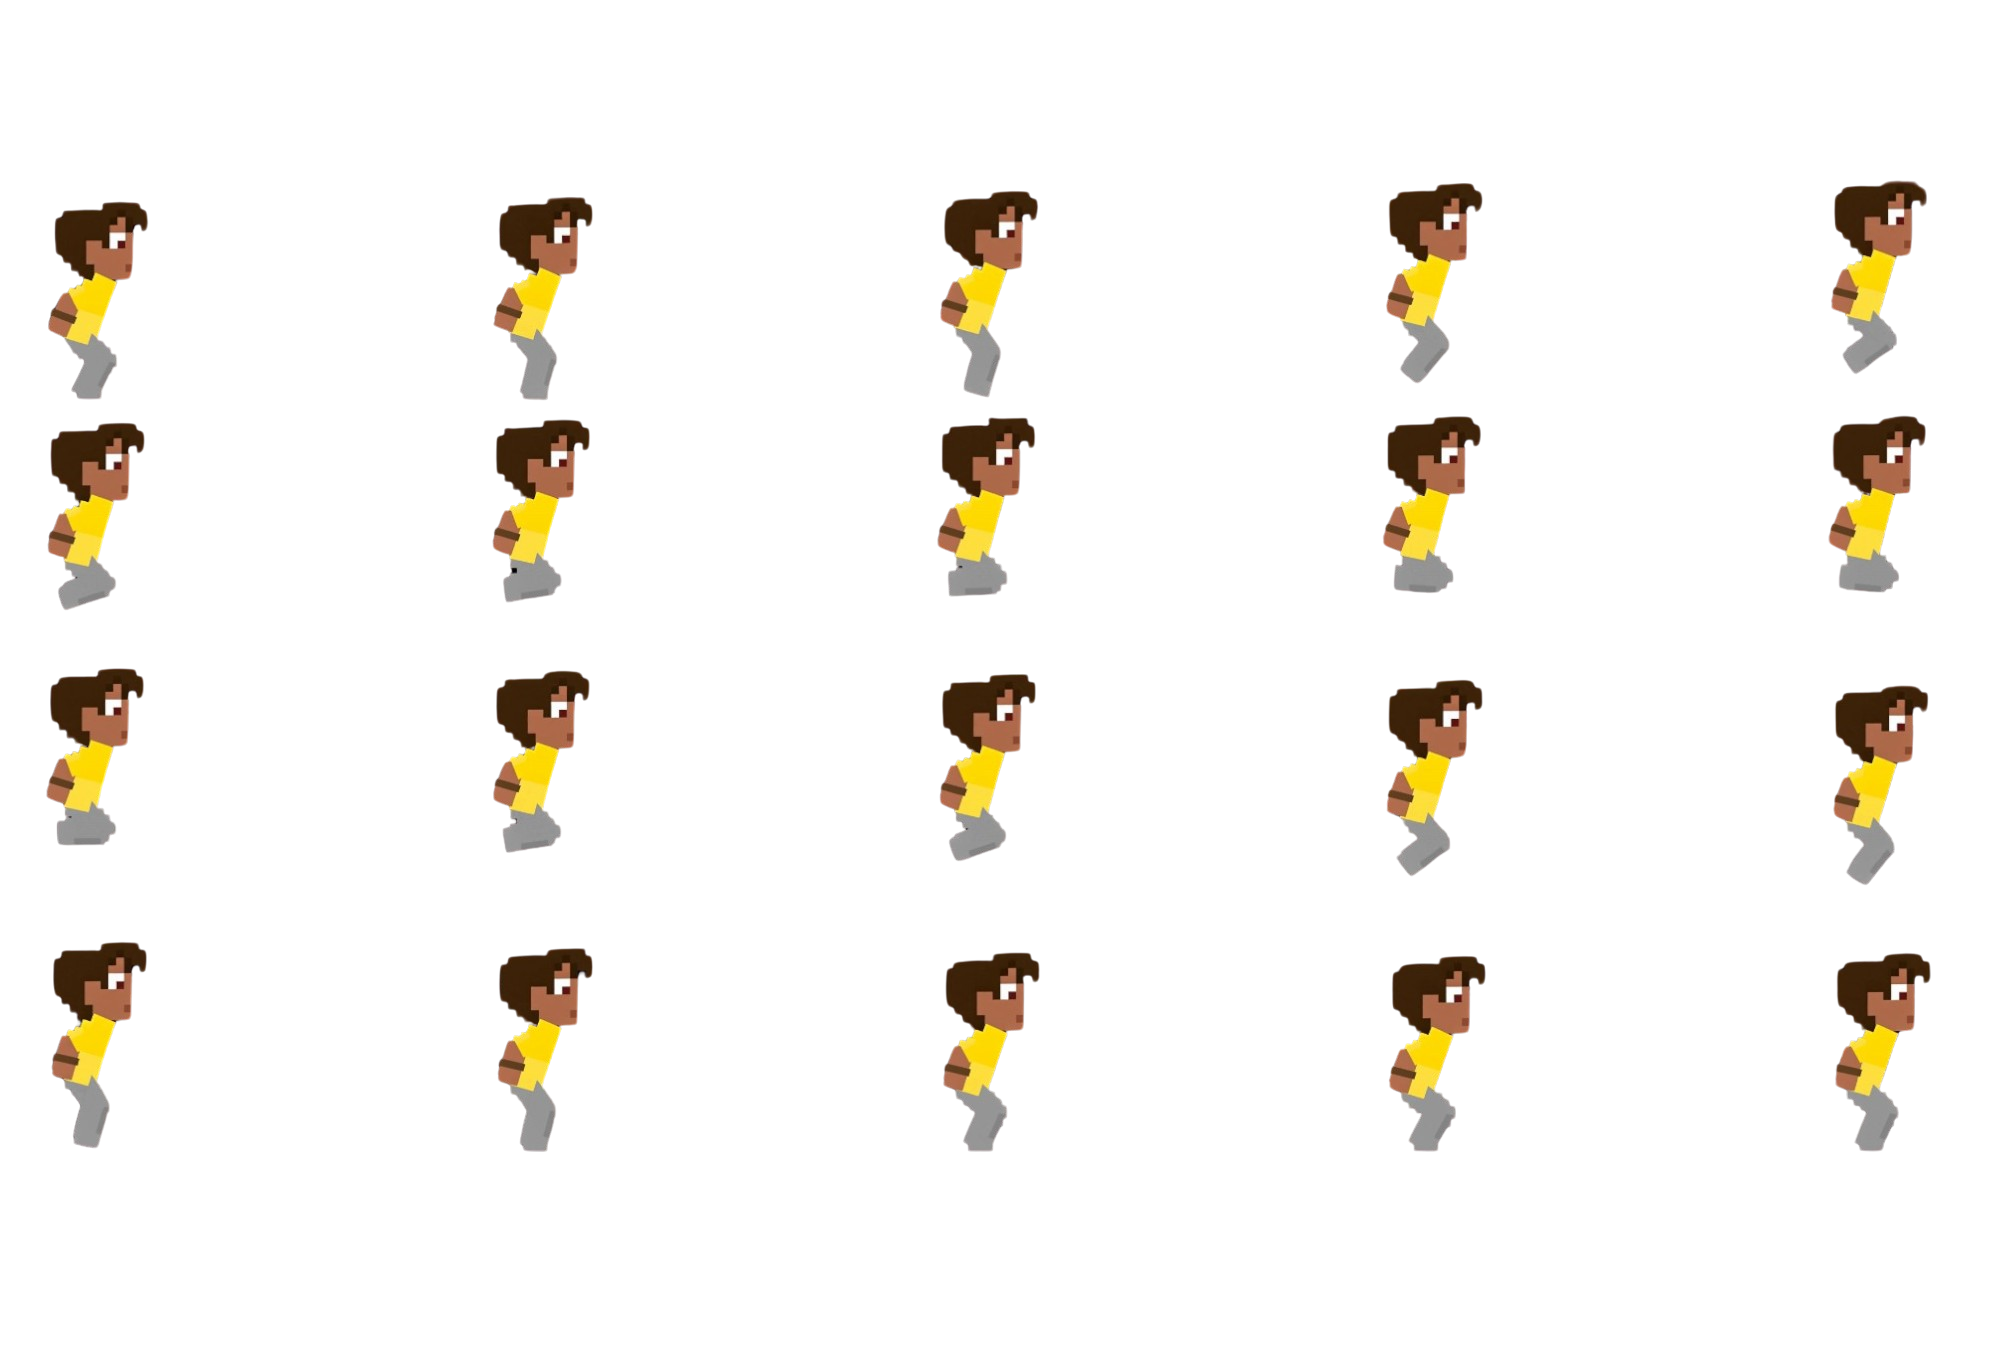
\includegraphics[width=0.8\linewidth]{figs/geminiPro/sprite sheet/jump_transparente.png}
    \legend{\small Fonte: Elaborada pela autora, utilizando a ferramenta ezgif.}
\end{figure}

Analisando todos os resultados, é possível notar que o uso do sprite no padrão pixel perfect fez com que a ferramenta conseguisse parcialmente manter uma coerência com o estilo de pixel art durante a animação, fazendo quadrados diagonais em vez de uma reta diagonal em certas partes do corpo. Essa tentativa de manter a animação como pixel art possui suas imperfeições, sendo feita apenas uma reta diagonal de 1 pixel independente do ângulo. 

% tipo, tem como fazer 2 pixels, sobe um, 2 pixels lado, sobe um
% Suponha que - e _ são pixeis em alturas diferentes
%Reta de 1 pixel = _-
%Reta de 2 pixels = __--